\documentclass[letterpaper,pdftex]{article}

\setlength{\textwidth}{168mm}
\setlength{\textheight}{210mm}
\setlength{\oddsidemargin}{0cm}
\setlength{\topmargin}{0cm}
\setlength{\headheight}{48pt}
\addtolength{\textheight}{-25pt}
\voffset -0.5in

\usepackage{natbib}
\usepackage[utf8]{inputenc}
\usepackage[spanish]{babel}
\usepackage{xcolor,graphicx}
\usepackage{fancyhdr}
\usepackage{multirow}
\usepackage{siunitx}
\usepackage{hyperref}
\hypersetup{
    colorlinks,
    citecolor=blue,
    filecolor=black,
    linkcolor=blue,
    urlcolor=black
}
\usepackage{epstopdf}
\usepackage[autolinebreaks,useliterate]{mcode}
\pagestyle{fancy}
\renewcommand{\headrule}{\color{gray}
\hrule width\headwidth height\headrulewidth \vskip-\headrulewidth}
\renewcommand{\footrule}{{\color{gray}
\vskip-\footruleskip\vskip-\footrulewidth
\hrule width\headwidth height\footrulewidth\vskip\footruleskip}}
\renewcommand{\headrulewidth}{1.5pt}
\renewcommand{\footrulewidth}{1.5pt}

\usepackage{caption}
\usepackage{subcaption}

\spanishdecimal{.}

\begin{document}
\fancyhead{}
\fancyfoot{}
\fancyhead[L]{
\begin{minipage}{3.5cm}
\begin{center}
	
\includegraphics[width=0.95\textwidth]{logousb.png}
\end{center}
\end{minipage}
\begin{minipage}{12cm}
\begin{flushleft}
\small \textsc{Universidad de San Buenaventura}\\
\small \textsc{Facultad de Ingeniería}\\
\small \textsc{Programa de Ingeniería Mecatrónica\\}
\end{flushleft}
\end{minipage}
}
\fancyhead[R]{
\begin{minipage}{3.0cm}
\begin{flushright}
\small \textsc{Mechanics of Materials \\ 2nd Term}\\
\small \textsc{2021-II}
\end{flushright}
\end{minipage}
}
\fancyfoot[R]{\large \textbf{\thepage}}

\begin{minipage}{0.3\textwidth}
\begin{flushleft}
\textbf{Author:}\\
\textit{Nikolay Prieto Ph.D(c)}\\
\end{flushleft}
\end{minipage}
\begin{minipage}{0.7cm}
\textcolor{gray}{\rule{0.3cm}{2.5cm}}
\end{minipage}
\begin{minipage}{0.64\textwidth}
\Large{\textbf{Computational Laboratory \\ ANSYS (Part I)}}
\end{minipage}\\

\noindent
\textcolor{gray}{\rule{\textwidth}{0.5pt}}\\
\renewcommand{\tablename}{Tabla}
\renewcommand{\arraystretch}{1.2}
\renewcommand\contentsname{Contenido}
\tableofcontents

\noindent
\textcolor{gray}{\rule{\textwidth}{0.5pt}}\\

\section{Introduction}

Discrete mathematics techniques allowed to approximate physical mechanical environments into computational models to find the reactions to those boundary conditions.  
% this was copied, edit!
The finite element method requires the system geometry to be defined by a number of points in space called nodes. Each node has a set of degrees of freedom (temperature, displacements, etc.) that can vary based on the inputs to the system. These nodes are connected by elements that define the mathematical interactions of the degrees of freedom (DOFs).

\subsection{Basic procedure for Finite element Analysis}

There are 10 basic steps in any FEA. First, the solid model geometry is created, the element type(s) and material properties are defined, and the solid model geometry is meshed to create the finite element model. In ANSYS, these steps are performed in the Preprocessor (PREP). Next, loads and constraints are applied, solution options are defined, and the problem is solved. These steps are performed in the solution processor (SOL). After the solution is ready, the results are plotted, viewed, and exported in one of the postprocessors (POST). Finally, the results are compared to first-order estimates, closed-form solutions, mathematical models, or experimental results to ensure that the output of the program is reasonable and as expected

\begin{itemize}
\item Define the solid model geometry \textit{(PREP)}
\item Select the element types. \textit{(PREP)}
\item Define the material Properties.\textit{(PREP)}
\item Mesh. \textit{(PREP)}
\item Define the boundary conditions. \textit{(SOL)}
\item Define the loads \textit{(SOL)}
\item Set the solution options \textit{(SOL)}
\item Solve \textit{(SOL)}
\item Plot, view, and Export the results \textit{(POST)}
\item Compare and Verify the results \textit{(POST)}

\end{itemize}

\subsection{ANSYS is an Engineering Software, not an engineer!}

As with all computer programs, the quality of your results will depend on the quality of your model. This includes the accuracy of the material properties, the appropriateness of the material models, how closely the simulated geometry and loads match the actual geometry and loads, and the validity of the simplifications and assumptions made. In general terms, Garbage In \--- Garbage Out. Finite element software programs can be thought of as very sophisticated calculators that help you to analyze engineering systems that could not otherwise be evaluated. They integrate the section properties of the system with the material properties to generate the equations to be solved. They convert the applied loads to the appropriate forms and apply them to the specified DOFs. They solve the generated system of equations. And, they help you to visualize and understand the results. But a finite element program will not comment on the validity of any assumptions made in setting up the model as long as the laws of physics are not violated. It also will not ensure that you are using the correct laws of physics for a given problem. Any errors that the program reports will be associated with the use of the program, and not with the physical or analytical system. In addition, it will not provide any commentary on the quality or implications of the results. Finite element software is only a tool. In the end, you, and you alone, are responsible for determining whether or not the results of your finite element model can be used to make or justify engineering decisions.

\subsection{Physics Capabilities}

Structural analyses may include linear and nonlinear buckling; fracture; composites; fatigue; and contact with and without friction, gaskets, joints, pretension, and spot welds. They can involve geometric non-linearities such as large strain and large deflection, and may use linear and non-linear material models including rate-dependent and rate-independent plasticity, hyper-elasticity, visco-elasticity, and creep. Structural analyses where time is important but time steps are very short, such as high-speed impacts and explosions, should be performed using one of the ANSYS explicit dynamics products such as ANSYS LS-DYNA or ANSYS AUTODYN.

\section{Static Axial Loading of a Notched plate in tension.}

In this exercise, you will perform a steady-state structural analysis of a notched rectangular plate that is loaded axially in tension. The plate is made of 6061-T6 aluminum with a Young’s modulus of $73.1$ GPa and a Poisson’s ratio of $0.33$. It is 15 cm wide and 10 cm tall with 1 cm diameter notches on each side. The notches are centered horizontally on the plate midplane and centered vertically on the upper and lower plate edges (Figure 2-1-1). The plate is thin so this can be treated as a two-dimensional (2D) problem. The geometry will be created using top down solid modeling techniques including Boolean operations.

A load of $1$ MPa will be placed on the right edge of the plate. The left edge of the plate will be constrained in $x$. This constraint will create a reaction force that will act as the second $1$ MPa load on the left. The plate will deform under the applied load, growing longer and thinner. This will force the notches to become ovals and a stress concentration will appear near the center of each notch.
The ratio of the height of the plate ($10$ cm) to the diameter of the notches ($1$ cm) is $10$ to $1$. Thus, the expected elastic stress concentration $Kt = \frac{\sigma_{\max}}{\sigma_{nom}}$ for this problem is $2.735$ and the expected gross stress concentration $Kg = \frac{\sigma_{\max}}{\sigma_{gross}}$ for this problem is $3.03$.

\begin{figure}[h]
   \centering
   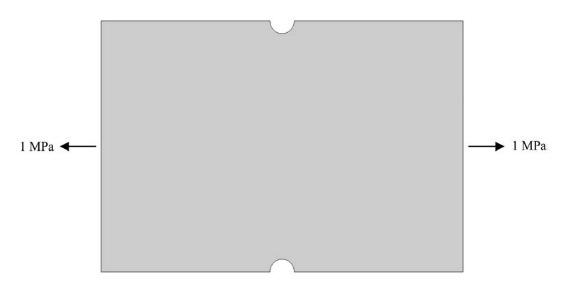
\includegraphics[width=0.6\textwidth]{notchedplate}
   \caption{Schematic view of the Notched plate under static conditions.}
   \label{fig:notchedplate}
\end{figure}

\subsection{Model Attributes}

\begin{itemize}
\item Young's Modulus $7.310 \times 10^10$ Pa
\item Poisson's ratio $\upsilon = 0.33$
\item Load 1 MPa on the right edge of the plate
\item Constrain 1: No displacement on the left edge in horizontal direction ($x$)
\item Constrain 2: No displacement of the lower left corner of the plate in the vertical ($y$) direction.
\end{itemize}


\section{Structural Analysis of a simple Warren Truss Using Direct Generation}

In this exercise, you will create a finite element model of a simple Warren truss using direct generation of the nodes and elements. The truss is 20 in. wide and 10 in. tall. Each member has a 1x1 in. cross section (Figure \ref{fig:warrentruss}).
%
The model will be built using the US customary system. The truss is made of aluminum  6061-O with a Youg Modulus  $E=1\times10^7$ \text{psi} and a Poisson’s ratio of $0.33$.

The truss will be modeled using spar (truss) elements. This allows uniaxial tension and compression within the members, but no bending of the members. All joints are pinned and can rotate freely. The pin in the lower left corner of the truss is fixed in space. The lower right corner of the truss is supported by rollers. A downward force of 1000 lb-f is applied to the bottom center joint of the truss. Because there are no out-of-plane boundary conditions, the truss will be modeled in 2D.
Given these assumptions and boundary conditions, the truss is statically determinate. All displacements and forces can be calculated by hand. Selected results are calculated at the end of the exercise for verification.


\begin{figure}[h]
   \centering
   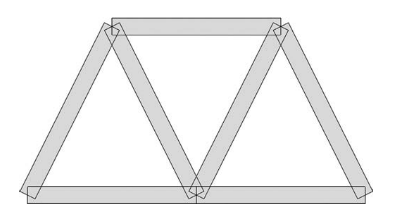
\includegraphics[width=0.6\textwidth]{truss_example}
   \caption{Schematic view of the Warren truss.}
   \label{fig:warrentruss}
\end{figure}

\subsection{Model Attributes}

\begin{itemize}
\item Young's Modulus $1 \times 10^7$ \text{psi}
\item Poisson's ratio $\upsilon = 0.33$
\item Load 1000 lb-f downward load on the lower center joint Constraints.
\item Constrain 1: No displacement on the lower right corner of the truss.
\item Constrain 2: No displacement on the lower left corner of the truss in the vertical direction.
\item Constrain 3: No out-of-plane displacements
\end{itemize}

\section{Activity}

Consider the truss structure shown in Fig. \ref{fig:trussex}. Constrains in $x$ and $y$ are presented in the diagram, The force application point is applied at the bottom right side downwards. 

\begin{figure}[h]
   \centering
   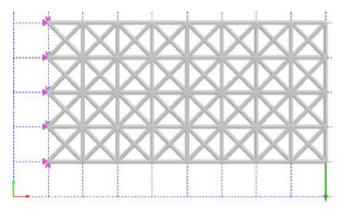
\includegraphics[width=0.6\textwidth]{Structure}
   \caption{Schematic view of one proposed design.}
   \label{fig:trussex}
\end{figure}

\subsection{Model Attributes}

\begin{itemize}
\item Young's Modulus $200$ \si{\GPa}
\item Material: Steel
\item Poisson's ratio $\upsilon = 0.33$
\item The minimum Cross-sectional area of each truss is $25 \si{\mm} \times 25 \si{\mm}$, however, you can modify this area in whatever truss of the structure so that obtain the lightest weight as possible.
\item Consider a maximal length and height of $3\si{\m} \times 1.5\si{\m}$   
\item Load 2 \si{\kN} downward load on the bottom right joint.
\item Constrain 1: No displacement on the the horizontal axis($x$) on the lower left line nodes.
\item Constrain 2: No displacement on the lower left line of the truss in the vertical direction.
\item Constrain 3: No out-of-plane displacements
\item Consider a Factor of Safety $FS=2.0$
\end{itemize}

Your task is to find a combination so that the truss is the lightest in consideration of the max stress obtained (including $FS$). An example is given in Fig. \ref{fig:opt_struc}


\subsection{Assignment requirements}

\begin{itemize}
\item The work is by pairs
\item Write a formal report i.e latex, word, Google Office, etc.
\item Establish the methods step by step.
\item Write your results in plots, short tables and short paragraphs.
\item Write the final weight and stress of the design given. Propose at least three options.
\item If you accomplish the previous requirements, your grade will be assign according to the minimum weight overall.
\end{itemize}


\begin{figure}[h]
   \centering
   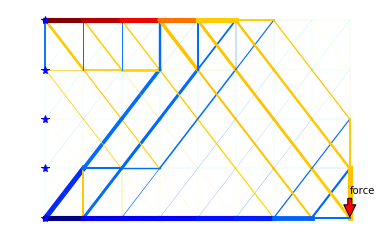
\includegraphics[width=0.6\textwidth]{output_22_3}
   \caption{Schematic view of the proposed structure.}
   \label{fig:opt_struc}
\end{figure}
\end{document}
